\documentclass[tikz]{standalone}
\usetikzlibrary{shapes,arrows.meta}
\begin{document}
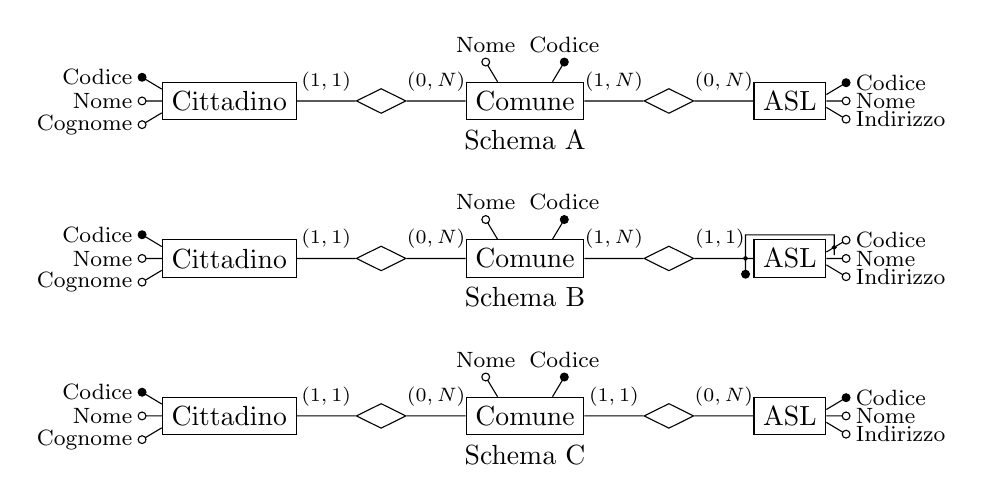
\begin{tikzpicture}
    \draw

    %%* Attributi:
    %%  node[draw, circle, inner sep=1pt, fill=black]{}node[right]{\footnotesize A}
    %%? Distanza orizzontale: E -(0.25,0.x)- A
    %%? Distanza verticale: E -(0,x * 0.22)- A

    %%* Cardinalità:
    %%  node[below right]{\scriptsize $(0,N)$}
    %%  node[above right]{\scriptsize $(0,N)$}
    %%  node[midway, above]{\scriptsize $(0,N)$}

    %%* Relazione:
    %%  node[draw, diamond, shape aspect=2, inner sep=3pt, anchor=90](r1){}
    %%  node[draw, diamond, shape aspect=2, inner sep=0.2pt, anchor=180](r2){R2}

    %%* Entità:
    %%  node[draw, rectangle, anchor=90](e1){}
    %%? Distanza verticale: E -(0.3)- R -(0.3) E
    %%? Distanza orizzontale: E -(0.75)- R -(0.75)- E

    %%* Schema A

    (0,0)node[draw, rectangle, anchor=180](e1){Cittadino}
    (e1.190)--++(-0.25,-0.15)node[draw, circle, inner sep=1pt, fill=white]{}node[left]{\footnotesize Cognome}
    (e1.180)--++(-0.25,0)node[draw, circle, inner sep=1pt, fill=white]{}node[left]{\footnotesize Nome}
    (e1.170)--++(-0.25,0.15) node[draw, circle, inner sep=1pt, fill=black]{}node[left]{\footnotesize Codice}

    (e1.0)--++(0.75,0)node[draw, diamond, shape aspect=2, inner sep=3pt, anchor=180](r1){}node[midway, above]{\scriptsize $(1,1)$}
    (r1.0)--++(0.75,0)node[draw, rectangle, anchor=180,label=below:{Schema A}](e1){Comune}node[midway, above]{\scriptsize $(0,N)$}
    (e1.145)--++(-0.15,0.25)node[draw, circle, inner sep=1pt, fill=white]{}node[above]{\footnotesize Nome}
    (e1.35)--++(0.15,0.25) node[draw, circle, inner sep=1pt, fill=black]{}node[above]{\footnotesize Codice}


    (e1.0)--++(0.75,0)node[draw, diamond, shape aspect=2, inner sep=3pt, anchor=180](r1){}node[midway, above]{\scriptsize $(1,N)$}
    (r1.0)--++(0.75,0)node[draw, rectangle, anchor=180](e1){ASL}node[midway, above]{\scriptsize $(0,N)$}
    (e1.350)--++(0.25,-0.15)node[draw, circle, inner sep=1pt, fill=white]{}node[right]{\footnotesize Indirizzo}
    (e1.0)--++(0.25,0)node[draw, circle, inner sep=1pt, fill=white]{}node[right]{\footnotesize Nome}
    (e1.10)--++(0.25,0.15) node[draw, circle, inner sep=1pt, fill=black]{}node[right]{\footnotesize Codice}


    %%* Schema B

    (0,-2)node[draw, rectangle, anchor=180](e1){Cittadino}
    (e1.190)--++(-0.25,-0.15)node[draw, circle, inner sep=1pt, fill=white]{}node[left]{\footnotesize Cognome}
    (e1.180)--++(-0.25,0)node[draw, circle, inner sep=1pt, fill=white]{}node[left]{\footnotesize Nome}
    (e1.170)--++(-0.25,0.15) node[draw, circle, inner sep=1pt, fill=black]{}node[left]{\footnotesize Codice}

    (e1.0)--++(0.75,0)node[draw, diamond, shape aspect=2, inner sep=3pt, anchor=180](r1){}node[midway, above]{\scriptsize $(1,1)$}
    (r1.0)--++(0.75,0)node[draw, rectangle, anchor=180,label=below:{Schema B}](e1){Comune}node[midway, above]{\scriptsize $(0,N)$}
    (e1.145)--++(-0.15,0.25)node[draw, circle, inner sep=1pt, fill=white]{}node[above]{\footnotesize Nome}
    (e1.35)--++(0.15,0.25) node[draw, circle, inner sep=1pt, fill=black]{}node[above]{\footnotesize Codice}


    (e1.0)--++(0.75,0)node[draw, diamond, shape aspect=2, inner sep=3pt, anchor=180](r1){}node[midway, above]{\scriptsize $(1,N)$}
    (r1.0)--++(0.65,0)node[midway, above]{\scriptsize $(1,1)$}node[draw, circle, inner sep=0.5pt, fill=black](a){}--++(0.1,0)node[draw, rectangle, anchor=180](e1){ASL}
    (e1.350)--++(0.25,-0.15)node[draw, circle, inner sep=1pt, fill=white]{}node[right]{\footnotesize Indirizzo}
    (e1.0)--++(0.25,0)node[draw, circle, inner sep=1pt, fill=white]{}node[right]{\footnotesize Nome}
    (e1.10)--++(0.1,0.06)node[draw, circle, inner sep=0.5pt, fill=black](b){}--++(0.15,0.09) node[draw, circle, inner sep=1pt, fill=white]{}node[right]{\footnotesize Codice}

    (a)++(0,-0.2)node[draw, circle, inner sep=1pt, fill=black]{}--++(0,0.5)-|(b)--++(0,-0.1)

    %%* Schema C

    (0,-4)node[draw, rectangle, anchor=180](e1){Cittadino}
    (e1.190)--++(-0.25,-0.15)node[draw, circle, inner sep=1pt, fill=white]{}node[left]{\footnotesize Cognome}
    (e1.180)--++(-0.25,0)node[draw, circle, inner sep=1pt, fill=white]{}node[left]{\footnotesize Nome}
    (e1.170)--++(-0.25,0.15) node[draw, circle, inner sep=1pt, fill=black]{}node[left]{\footnotesize Codice}

    (e1.0)--++(0.75,0)node[draw, diamond, shape aspect=2, inner sep=3pt, anchor=180](r1){}node[midway, above]{\scriptsize $(1,1)$}
    (r1.0)--++(0.75,0)node[draw, rectangle, anchor=180,label=below:{Schema C}](e1){Comune}node[midway, above]{\scriptsize $(0,N)$}
    (e1.145)--++(-0.15,0.25)node[draw, circle, inner sep=1pt, fill=white]{}node[above]{\footnotesize Nome}
    (e1.35)--++(0.15,0.25) node[draw, circle, inner sep=1pt, fill=black]{}node[above]{\footnotesize Codice}


    (e1.0)--++(0.75,0)node[draw, diamond, shape aspect=2, inner sep=3pt, anchor=180](r1){}node[midway, above]{\scriptsize $(1,1)$}
    (r1.0)--++(0.75,0)node[draw, rectangle, anchor=180](e1){ASL}node[midway, above]{\scriptsize $(0,N)$}
    (e1.350)--++(0.25,-0.15)node[draw, circle, inner sep=1pt, fill=white]{}node[right]{\footnotesize Indirizzo}
    (e1.0)--++(0.25,0)node[draw, circle, inner sep=1pt, fill=white]{}node[right]{\footnotesize Nome}
    (e1.10)--++(0.25,0.15) node[draw, circle, inner sep=1pt, fill=black]{}node[right]{\footnotesize Codice}

    ;
\end{tikzpicture}
\end{document}